\subsubsection{Selección de la fuente de alimentación}

Se tienen en cuenta los diferentes parámetros que se plantearon en la sección anterior, se puede hacer la elección de diversos modelos de fuente de alimentación, cada una de las fuentes consultadas,posee características distintas, aunque solo se encuentran de voltaje fijo, por lo que es necesaria realizar el acoplamiento de las diferentes fuentes de alimentación (Tabla \ref{tab:fuentesali}).

        \begin{table}[h!]
            \begin{center}
            \caption{Opciones de alimentación eléctrica}
                \begin{tabular}{| c | c | c | c |}
                    \hline
                    Fuente & Voltaje & Amperaje & Precio  \\ \hline
                    Eliminador & 5 VDC & 3 A & \$ 80.00  \\
                    Eliminador & 12 VDC & 2 A & \$ 80.00  \\ \hline  
                \end{tabular}
            
            \label{tab:fuentesali}
        \end{center}
    \end{table}

Estos elementos están conectados a un multicontacto, desde donde se distribuye la energía eléctrica del sistema. Este multicontacto, tendrá al menos 6 terminales para los 2 eliminadores, la bomba de agua, la resistencia y los 2 motores.

En este punto, es muy importante seleccionar un multicontacto con una cable de alimentación que sea capaz de soportar al menos 10 A para los sistemas internos del compostador, principalmente la corriente del sistema de temperatura y el motor de aireación.

Para el proyecto se han revisado algunas opciones y la que más se acerca a las necesidades del proyecto, se puede encontrar un multicontacto industrial de la marca Volteck, el modelo MUL-612X (Figura \ref{fg:multicontacto}).

Este cuenta con 6 conectores disponibles para transmitir una tensión de 127 V AC con una corriente de 15 A. Con estos requerimientos se puede suministrar la alimentación a todos los subsistemas del compostador. 

\begin{figure}[h!]
            \centering
            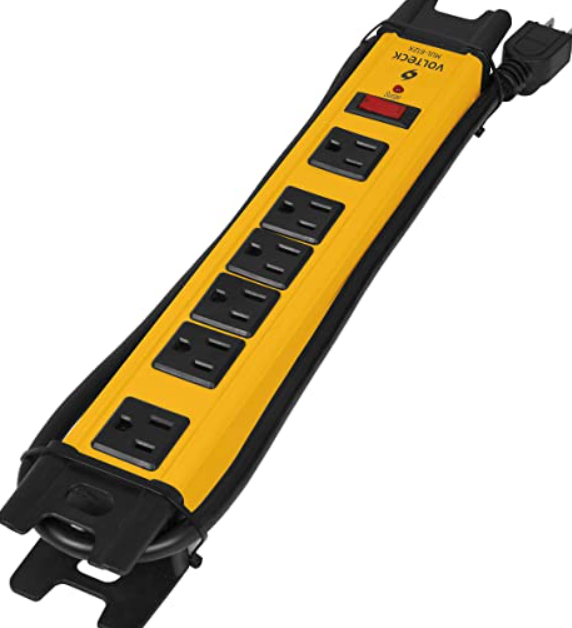
\includegraphics[scale=0.2]{images/Capitulo 4/S3/extens.png}
            \caption{Multicontacto uso industrial}
            \label{fg:multicontacto}
\end{figure}

\newpage 

